\documentclass{article}

\usepackage[a4paper, hmargin={20mm, 20mm}, vmargin={25mm, 30mm}]{geometry}
\usepackage[utf8]{inputenc}
\DeclareUnicodeCharacter{0301}{\'{e}} %erro do UNICODE
\usepackage[english, main=portuguese]{babel}

\usepackage[hidelinks]{hyperref}
\usepackage{bookmark}
\usepackage{cancel}
\usepackage{comment}

\usepackage{array}
\usepackage{indentfirst}
\usepackage{multicol}
\usepackage{subfiles}

\usepackage{wrapfig}
\usepackage{graphicx}
\usepackage{subcaption}
\graphicspath{ {./imagens/} }

\usepackage{titlesec}

\usepackage{amsmath}
\usepackage{esdiff}
\usepackage{float}
\usepackage{enumitem}
\restylefloat{table}

%\titleformat{<command>}[<shape>]{<format>}{<label>}{<sep>}{<before-code>}[<after-code>]
\titleformat
{\section} %comand
[block]  %shape
{\normalfont\LARGE} %format
{\thesection. } %label
{0mm} %sep
{} %before-code
[{\titlerule[0.1mm]}] %after-code

\titlespacing*{\section}{0mm}{0mm}{10mm}

\titleformat
{\subsection} %comand
[block]  %shape
{\normalfont\large} %format
{\thesubsection. } %label
{0mm} %sep
{} %before-code
[] %after-code

\titlespacing*{\subsection}{0mm}{5mm}{2.5mm}



\begin{document}
\begin{titlepage}
    \begin{center}
        \rule{450pt}{0.5pt}\\[4mm]
        {\Huge EM360 - Termodinâmica I}\\
        \rule{450pt}{0.5pt}\\[2mm]
        {\Large Resumo Teórico}\\[200mm]
        \today\\
        \rule{250pt}{0.5pt}\\
        {\large Guilherme Nunes Trofino}\\
        {\large 217276}\\
    \end{center}
\end{titlepage}
\newpage

        \tableofcontents
    \newpage

    \section{Apresentação}
        \paragraph{Arquivo}Este documento, escrito em \LaTeX, é um resumo para a disciplina EM360 - Termodinâmica I de autoria de Guilherme Nunes Trofino que poderá ser encontrado no seguinte repositório do \href{https://github.com/tr0fin0/classes}{GitHub}. Não me responsabilizo pela utilização do documento, que pode apresentar erros, e agradeço se problemas forem reportados. 
\newpage

    \section{Introdução}
        \subsection{Sistema}
            \paragraph{Definição}Região, ou objeto, a ser estudado, serparado da \textbf{Vizinhança} por sua \textbf{Fronteira}, onde as variáveis são conhecidas. Estes são classificados de acordo com a mobilidade, ou não, de matéria e ou energia como descrito a seguir:
                \begin{enumerate}[noitemsep]
                    \item \textbf{Fechado}: Não há fluxo de matéria e há fluxo de energia:
                        \begin{enumerate}[noitemsep]
                            \item \textbf{Isolado}: Não há fluxo de matéria ou energia com a vizinhança;
                        \end{enumerate}
                    \item \textbf{Aberto}: Há fluxo de matéria e energia:
                        \begin{enumerate}[noitemsep]
                            \item \textbf{Volume de Controle}: Fronteira do sistema;
                        \end{enumerate}
                \end{enumerate}

        \subsection{Propriedade}
            \paragraph{Definição}Características macroscópias do sistema, independentes do \textbf{Histórico} de processos. Estas são classificadas de acordo com a dependência, ou não, da extensão da matéria como descrito a seguir:
                \begin{enumerate}[noitemsep]
                    \item \textbf{Extensiva} Dependente do objeto estudado, como:
                        \begin{enumerate}[noitemsep]
                            \item Massa;
                            \item Volume;
                            \item Energia;
                        \end{enumerate}
                    \item \textbf{Intensiva} Independente do obejto estudado, como:
                        \begin{enumerate}[noitemsep]
                            \item Massa Específica;
                            \item Volume Específico;
                            \item Temperatura
                        \end{enumerate}
                \end{enumerate}
            Qualquer propriedade intensiva poderá ser obtida a partir de sua equivalente extensiva divido pela massa associada ao sistema ou substância.

        \subsection{Processo}
            \paragraph{Definição}Procedimento que altera as \textbf{Propriedades}, com duas destas características pode-se determinar o estado da substância, do sistema. Estes são classificados de acordo com seu comportamento ao longo do tempo como descrito a seguir:

                \begin{enumerate}[noitemsep]
                    \item \textbf{Politrópico}: Proceso que relaciona pressão e volume pela expressão: $pV^{n} = c$;
                    \item \textbf{Adiabático}: Processo que não troca calor com a vizinhança;
                    \item \textbf{Quasestático}: Processo suficientemente lento considerado em equilíbrio;
                    \item \textbf{Regime Permanente}: Processo que não altera as propriedades do sistema;
                    \item \textbf{Ciclo}: Processo que retorna ao estado inicial;
                \end{enumerate}
                
                \begin{enumerate}[noitemsep]
                    \item \textbf{Isentrópico}: Processo que não varia de entropia;
                    \item \textbf{Isobárico}: Processo que não varia de pressão;
                    \item \textbf{Isotérmico}: Processo que não varia de temperatura;
                    \item \textbf{Isovolumétrico}: Processo que não varia de volume;
                \end{enumerate}

                \begin{enumerate}[noitemsep]
                    \item \textbf{Irreversível}: Sistema e sua Vizinhança não podem retornar, simultaneamente, a seus estados iniciais;
                    \item \textbf{Reversível}: Sistema e sua Vizinhança podem retornar, simultaneamente, a seus estados iniciais;
                    \item \textbf{Reversível Internamente}: Fronteira escolhida de tal forma que não hajam irreversibilidades no sistema;
                \end{enumerate}
\newpage

        \subsection{Unidades SI}
            \paragraph{Definição}Utiliza-se unidades do sistema internacional para as descrições de fórmulas. Estas são as unidades utilizadas com suas respectivas representações:
                \begin{table}[h]
                    \centering
                    \begin{tabular}{llc}\hline
                        Quantidade & Unidades                                     & Símbolo\\[1mm]\hline
                        Força      & kg m/s\textsuperscript{2}                    & N\\
                        Pressão    & kg/ms\textsuperscript{2}                    & Pa\\
                        Energia    & kg m\textsuperscript{2}/s\textsuperscript{2} & J\\
                        Potência   & kg m\textsuperscript{2}/s\textsuperscript{3} & W\\\hline
                    \end{tabular}
                \end{table}
\newpage

    \section{Definições Básicas}
        \subsection{Pressão}
            \paragraph{Definição}Força normal exercida por um corpo, ou fluido, sobre uma superfície. Formalmente descrito pela seguinte equação:
                \[\boxed{p = \diff{F_{\text{normal}}}{A} \hspace{5mm} \left[\text{Pa} = \frac{\text{kg}}{\text{m}\text{ s}^{2}}\right]}\]
                \[1 \text{ atm} = 101325 \text{ Pa} \hspace{5mm} 1 \text{ bar} = 10^5 \text{ Pa}\]

        \subsection{Volume Específico}
            \paragraph{Definição}Volume ocupado por unidade de masssa, inverso da densisdade. Formalmente descrito pela seguinte equação:
                \[\boxed{\nu = \rho^{-1} = \diff{v}{m} \hspace{5mm} \left[\frac{\text{m}^{3}}{\text{kg}}\right]}\]

        \subsection{Temperatura}
            \paragraph{Definição}Quantidade calor associada um corpo ou fluido. Corpos com diferentes temperaturas $T_{1}$ e $T_{2}$ tendem, quando em contato, a estabilizar em valor intermediário, nomeado como \textbf{Equilíbrio Térmico}.

            \paragraph{Escalas}Há diferentes convenções térmicas normalizadas em três pontos comuns: \textbf{Ebulição da Água}, \textbf{Fusão da Água} e \textbf{Zero Absoluto}. 
                \[T[^{o}\text{C}] = T[\text{K}] - 273,15\]
                \[T[^{o}\text{F}] = 1,8T[^{o}\text{C}] + 32\]

        \subsection{Reservatórios Térmicos}
            \paragraph{Definição}Corpos suficientemente extensos em que pequenas alterações, com relação ao todo, em suas \textbf{Propriedades}, podem ser desprezadas. Este corpos apresentam apenas irreversibilidades internas.

        \subsection{Energia Interna}
            \paragraph{Definição}Toda energia não cinética e não potencial, normalmente composta por energia térmica, química, nuclear e radiante. Formalmente descrita pela seguinte equação:
                \[\boxed{U = u \cdot m \hspace{5mm} \left[\text{J} = \frac{\text{kg m}^{2}}{\text{ s}^{2}}\right]}\]

        \subsection{Entalpia}
            \paragraph{Definição}Representa a quantidade de energia transferida durante um processo em virtude de trabalho. Formalmente descrita pela seguinte equação:
                \[\boxed{H = \Delta U + p\Delta V \hspace{5mm} \left[\text{J} = \frac{\text{kg m}^{2}}{\text{ s}^{2}}\right]}\]

        \subsection{Energia Total}
            \paragraph{Definição}Somatório de todas as energias de uma substância, ou sistema, descrita em sua forma intensiva ou extensiva. Formalmente descrita pela equação:
                \[\boxed{E = mu + \frac{m V^{2}}{2} + mgz \hspace{5mm} \left[\text{J} = \frac{\text{kg m}^{2}}{\text{ s}^{2}}\right]}\]

        \subsection{Calor Específico}
            \paragraph{Definição}Capacidade de uma substância receber, ou ceder, calor para outra. Formalmente descrito, a \textbf{Volume} constante e a \textbf{Pressão} constante respectivamente, pelas seguintes equações:
                \[
                    \boxed{c_{\text{v}} = \diffp{u}{T}\Big|_{\text{v}} \hspace{5mm} \left[\frac{\text{kJ}}{\text{kg K}}\right]} \hspace{5mm}
                    \boxed{c_{\text{p}} = \diffp{h}{T}\Big|_{\text{p}} \hspace{5mm} \left[\frac{\text{kJ}}{\text{kg K}}\right]}
                \]

            \paragraph{Constante Adiabática}Razão entre o \textbf{Calor Específico} a pressão constante e a volume constante como a constante adiabática para que diferentes substâncias possam ser diretamente comparadas como:
                \[
                    \boxed{k = \frac{c_{\text{p}}}{c_{\text{v}}}}
                    \hspace{2,5mm}
                    \text{ quando $k = 1.4$, trata-se de \textbf{Gás Ideal};}\]

        \subsection{Calor}
            \paragraph{Definição}Quantificação do grau de mobilidade, consequemente troca energia, dos átomos pertencentes a uma substância. Formalmente descrita pela seguinte equação:
                \[
                    \boxed{Q = mc \Delta T \hspace{5mm} \left[\text{J} = \frac{\text{kg m}^{2}}{\text{s}^{2}}\right]}
                \]
            Normalmente gases esfriam quando expandem e esquentam quando comprimem. Além disso, calor pode se propagar por 3 mecanismos distintos a depender da interração com o ambiente:
                \begin{enumerate}[noitemsep]
                    \item Condução;
                    \item Convecção;
                    \item Radiação;
                \end{enumerate}

            \paragraph{Convenção}Define-se que o sistema, independente de seu desempenho, deverá receber calor:
                \begin{enumerate}[noitemsep]
                    \item $Q>0$: Sistema recebe calor da vizinhança;
                    \item $Q<0$: Sistema fornece calor à vizinhança;
                \end{enumerate}

        \subsection{Trabalho}
            \paragraph{Definição}Transferência de energia entre o sistema e sua vizinha, pela expansão ou contração do fluido, causada sobre a forma de energia cinética, potencial e ou interna. Formalmente descrito pelas seguintes equações, respectivamente para \textbf{Sistema Fechado} e \textbf{Volume de Controle}:
                \[
                    \boxed{
                        W =
                        \int^{V_{2}}_{V_{1}} pdV \hspace{5mm}
                        \left[\text{J} = \frac{\text{kg m}^{2}}{\text{s}^{2}}\right]}
                    \hspace{5mm}
                    \boxed{
                        \frac{\dot{W}}{\dot{m}} =
                        \int^{p_{2}}_{p_{1}} {vdp} \hspace{5mm}
                        \left[\frac{\text{J}}{\text{kg}} = \frac{\text{m}^{2}}{\text{s}^{2}}\right]}
                \]
            Onde:
                \begin{enumerate}[noitemsep]
                    \item Se $p_{1} > p_{2}$ ocorre expansão e, portanto, $W$ será positivo;
                    \item Se $p_{1} < p_{2}$ ocorre compressão e, portanto, $W$ será negativo;
                \end{enumerate}

            \paragraph{Convenção}Define-se que o sistema, independente de seu desempenho, deverá realizar trabalho:
                \begin{enumerate}[noitemsep]
                    \item $W>0$: Sistema realiza trabalho sobre a vizinhança;
                    \item $W<0$: Vizinhança realiza trabalho sobre o sistema;
                \end{enumerate}

            \paragraph{Processo Politrópico}Sistemas que podem ser modelados de acordo com a relação entre pressão e volume, $p V^{n} = c$ ou $p v^{n} = c$, obtido experimentalmente. Formalmente descrito pelas seguintes equações, respectivamente para \textbf{Sistema Fechado} e \textbf{Volume de Controle}:
                \[
                    \boxed{
                        W = \int_{V_{1}}^{V_{2}} \frac{c}{V^{n}} dV = 
                        \begin{cases}
                            n \neq 1, & \frac{p_{2} V_{2} - p_{1} V_{1}}{1-n}\\[4mm]
                            n = 1,    & p_{1} V_{1} \ln{\frac{V_{2}}{V_{1}}}
                        \end{cases}}
                    \hspace{5mm}
                    \boxed{
                        \frac{\dot{W}}{\dot{m}} = \int_{p_{1}}^{p_{2}} \frac{c^{1/n}}{p^{1/n}} dp = 
                        \begin{cases}
                            n \neq 1, & \frac{n(p_{2} v_{2} - p_{1} v_{1})}{1-n}\\[4mm]
                            n = 1,    & - p_{1} v_{1} \ln{\frac{p_{2}}{p_{1}}}
                        \end{cases}}
                \]

        \subsection{Entropia}
            \paragraph{Definição}Representa a desorganização do sistema, relacionando as influências dos processos no estado do sistema avaliado. Formalmente definida pela seguinte relação:
                \[\boxed{S_{2} - S_{1} = \int_{1}^{2}\left(\frac{\partial Q}{T}\right)_{\text{rev}} \hspace{5mm} \left[\frac{\text{J}}{\text{K}} = \frac{\text{kg m}^{2}}{\text{K s}^{2}}\right]}\]
            Onde $\partial Q$ representa do sistema trocado com sua vizinhança em sua fronteira e $T$ representa a temperatura absoluta do sistema.

            \paragraph{Modelo Tds}Assumindo substância pura e compressível, percorrendo um processo internamente reversível com efeitos da gravidade e movimento desprezíveis. Assim o balanço de energia, obtido pela 1\textsuperscript{a} Lei, será descrito pela seguinte equação:
                \[
                    \boxed{Tds = dU + pdV} \hspace{30mm} \boxed{Tds = dH - Vdp}
                \]

            \paragraph{Modelo Gás Ideal}Somado as considerações para o modelo Tds, considera-se, também, que a substância se comporta como gás ideal. Desta maneira a entropia será descrita pelas seguintes equações:
                \[
                    \boxed{s_{2} - s_{1} = \int_{T_{1}}^{T_{2}} \frac{c_{\text{v}}(T)}{T}dT + R \ln\left(\frac{V_{2}}{V_{1}}\right)} \hspace{5mm}
                    \boxed{s_{2} - s_{1} = \int_{T_{1}}^{T_{2}} \frac{c_{\text{p}}(T)}{T}dT + R \ln\left(\frac{p_{2}}{p_{1}}\right)}
                \]
            As tabelas termodinâmicas A22 e A23 fornecem valores calculados para a integral do calor específico a pressão constante, denotada como $s^{o}$. Desta maneira a entropia será descrita pela seguinte equação:
                \[s^{o}(T_{a}) = \int_{0}^{T_{a}} \frac{c_{\text{p}}(T)}{T}dT\]
                \[\boxed{s_{2} - s_{1} = s^{o}(T_{2}) - s^{o}(T_{1}) - R \ln\left(\frac{p_{2}}{p_{1}}\right)}\]
            Caso os calores específicos sejam constantes, independetes da temperatura da substância, a integral será trivial. Desta maneira a entropia será descrita pelas seguintes equações:
                \[
                    \boxed{s_{2} - s_{1} = c_{\text{v}} \ln\left(\frac{T_{2}}{T_{1}}\right) + R \ln\left(\frac{v_{2}}{v_{1}}\right)} \hspace{5mm}
                    \boxed{s_{2} - s_{1} = c_{\text{p}} \ln\left(\frac{T_{2}}{T_{1}}\right) + R \ln\left(\frac{p_{2}}{p_{1}}\right)}
                \]

            \paragraph{Modelo Incompressível}Assumindo substância incompressível com volume constante, percorrendo um processo internamente reversível com efeitos da gravidade e movimento desprezíveis. Desta maneira a entropia será descrita pela seguinte equação:
                \[\boxed{s_{2} - s_{1} = \int_{T_{1}}^{T_{2}} \frac{c_{\text{v}}(T)}{T} dT}\]
            Caso o calor específico a volume constante seja constante a integral será trivial. Desta maneira a entropia será descrita pelas seguint equação:
                \[\boxed{s_{2} - s_{1} = c_{\text{v}} \ln\left(\frac{T_{2}}{T_{1}}\right)}\]
\newpage

    \section{Diagramas de Estado}
        \paragraph{Definição}Representam como uma substância modifica seu estado de acordo com suas condições. Quando houver mistura entre os diferentes estados a seguinte notação será utilizada:
            \begin{enumerate}[noitemsep]
                \item \textbf{Líquido}: Apresentado com o subscrito \textit{f} quando em mistura;
                \item \textbf{Vapor}: Apresentado com o subscrito \textit{g} quando em mistura;
                \item \textbf{Mistura Líquido-Vapor}: Apresentado como \textit{L+V};
            \end{enumerate}

        \paragraph{Considerações}Aproximações de comportamento e variáveis do sistema podem ser tomando em certos cenários, descritos a seguir:
            \begin{enumerate}[noitemsep]
                \item \textbf{Processo Quasestático}: Expansão, ou compressão, que ocorrer lentamente no interior de um conjunto cilíndro pistão poderá desconsiderar a pressão causada pelo pistão;
                \item \textbf{Líquido Comprimido}: Líquidos sobre pressões inferiores a 25 bar, fora da condição de compressão, poderá ter suas propriedades aproximadas pelos valores do líquido saturado;
                    \[
                        \boxed{v(T, p) = v_{f}(T)} \hspace{5mm}
                        \boxed{u(T, p) = u_{f}(T)} \hspace{5mm}
                        \boxed{h(T, p) = h_{f}(T)} \hspace{5mm}
                        \boxed{s(T, p) = s_{f}(T)}
                    \]
            \end{enumerate}

            \begin{figure}[h]
                \begin{subfigure}[t]{0.5\textwidth}
                    \centering
                    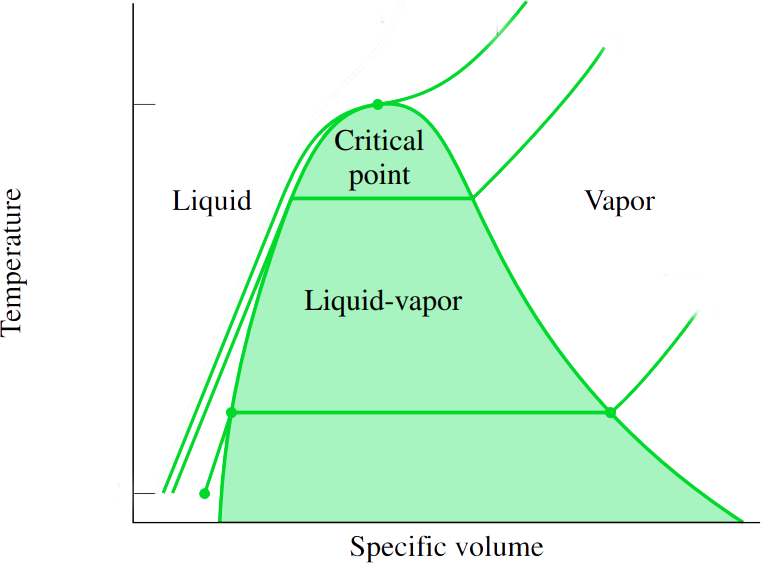
\includegraphics[height = 5cm]{D. Tv Completo.png}
                    \caption{Diagrama Temperatura Entropia}
                \end{subfigure}
                \begin{subfigure}[t]{0.5\textwidth}
                    \centering
                    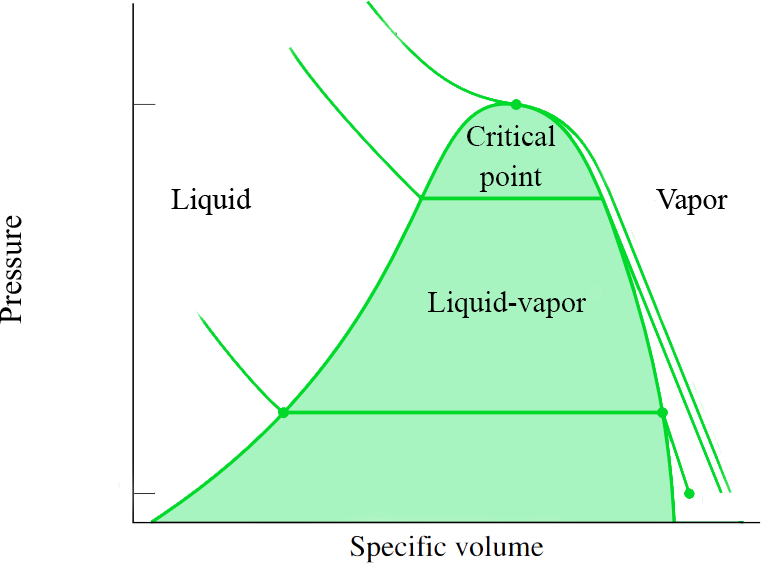
\includegraphics[height = 5cm]{D. pv Completo.png}
                    \caption{Diagrama Entalpia Entropia}
                \end{subfigure}
                \caption{Diagramas de Estado para Volume Específico}
            \end{figure}

            \begin{figure}[h]
                \begin{subfigure}[t]{0.5\textwidth}
                    \centering
                    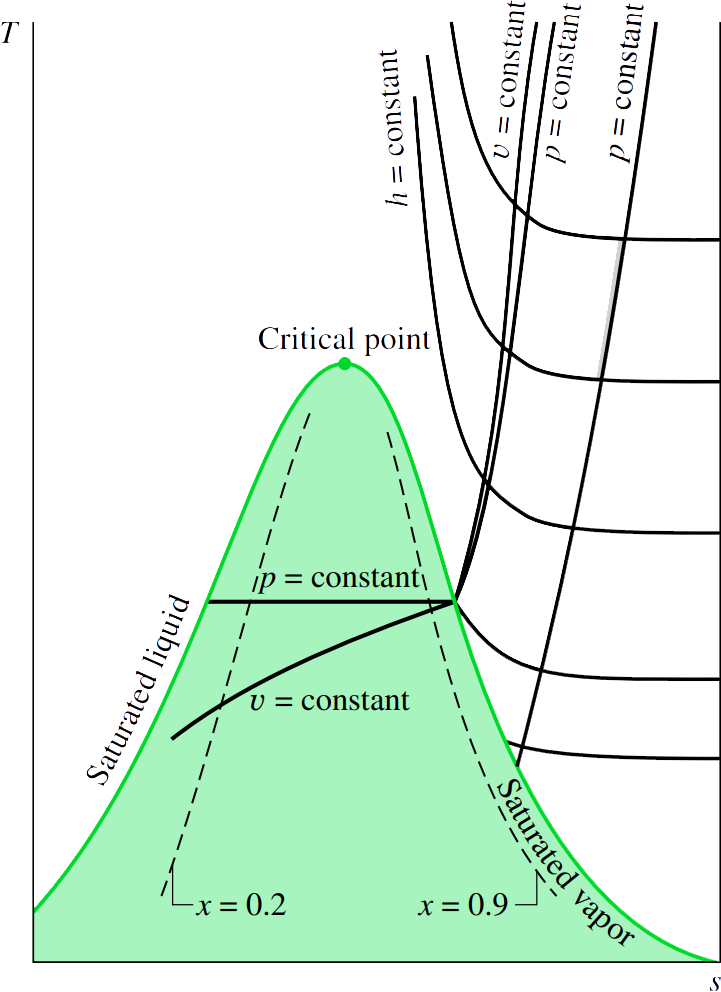
\includegraphics[height = 5cm]{D. Ts Comum.png}
                    \caption{Diagrama Temperatura Entropia}
                \end{subfigure}
                \begin{subfigure}[t]{0.5\textwidth}
                    \centering
                    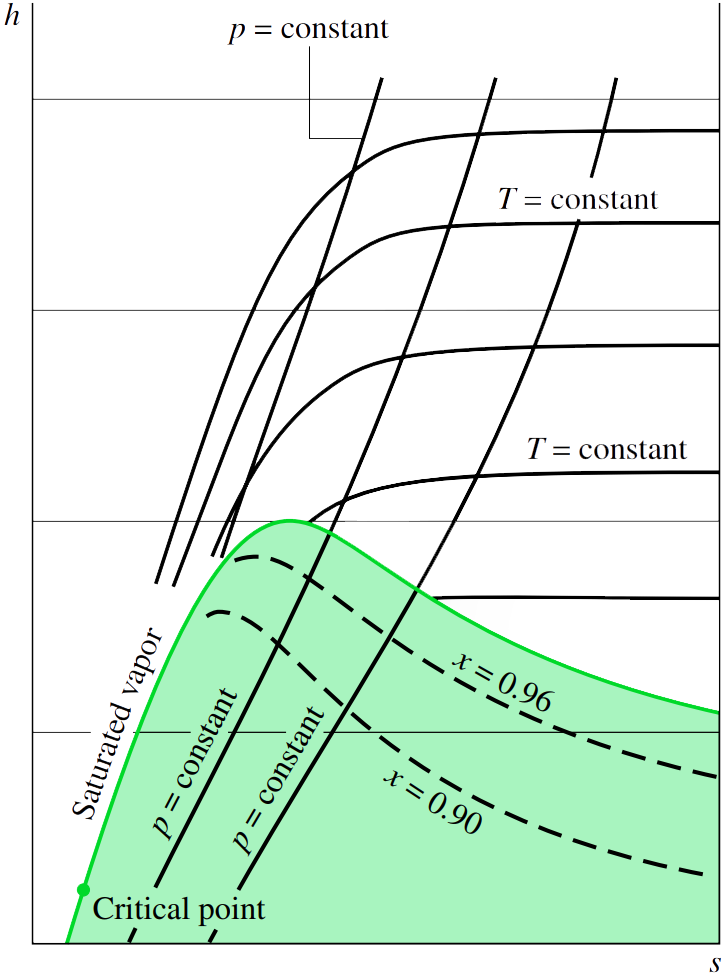
\includegraphics[height = 5cm]{D. hs Comum.png}
                    \caption{Diagrama Entalpia Entropia}
                \end{subfigure}
                \caption{Diagramas de Estado para Entropia}
            \end{figure}

        \subsection{Princípio do Estado}
            \paragraph{Definição}De acordo com a 1\textsuperscript{a} Lei, há duas formas de alterar a energia de fluido compressível em um sistema fechado, através do calor ou através do trabalho. Caso duas propriedades intensivas quaisqueres sejam fixadas não haverá processo e assim não haverá mudança de estado.

        \subsection{Tabelas de Propriedades}
            \paragraph{Definição}Certos fluidos possuem suas características físicas registradas a diferentes combinações de variáveis, como temperatura e pressão. Essas tabelas permitem, com a entrada de uma variável, encontrar as demais caractéristicas da substância avaliada.

            \paragraph{Tabelas}Desenvolvidas a partir das linhas de líquido saturado e vapor saturado, denotando as características a cada estado. Entre as principais tabelas para água temos:
                \begin{enumerate}[noitemsep]
                    \item \textbf{Tabela A2}: Entrada com Temperatura;
                    \item \textbf{Tabela A3}: Entrada com Pressão;
                    \item \textbf{Tabela A4}: Entrada com Pressão e Temperatura para Vapor Superaquecido;
                    \item \textbf{Tabela A5}: Entrada com Pressão e Temperatura para Líquido Comprimido;
                \end{enumerate}

        \subsection{Título de Mistura}
            \paragraph{Definição}Fração da propriedade avaliada na Mistura Líquido-Vapor, essencial para caracterizar o estado de tal composição. Formalmente descrita pela seguinte equação:
                \[\boxed{x = \frac{m_{g}}{m_{f} + m_{g}}}\]
            Com as propriedades específicas de uma Mistura L-V pode-se desenvolver importantes relações entre o título e a propriedade específica analisada.
                \[x = \frac{X}{m}
                    = \frac{X_{g} + X_{f}}{m_{g} + m_{f}}
                    = \frac{X_{g}}{m_{f} + m_{g}} + \frac{X_{f}}{m_{f} + m_{g}}
                    = \underbrace{\left(\frac{X_{g}}{m_{g}}\right)}_{\text{$ = x_{g}$}} \frac{m_{g}}{m_{f} + m_{g}} + \underbrace{\left(\frac{X_{f}}{m_{f}}\right)}_{\text{$ = x_{f}$}} \frac{m_{f}}{m_{f} + m_{g}}\]
                \[\boxed{v = x \cdot x_{g}+(1-x)x_{f}}\]
            Caso seja necessário obter o título com base nas propriedades físicas analisadas basta rearranjar algebricamente a última equação para obter o que segue.
                \[\boxed{x = \frac{v - x_{f}}{x_{g} - x_{f}}}\]
                \begin{figure}[h]
                    \centering
                    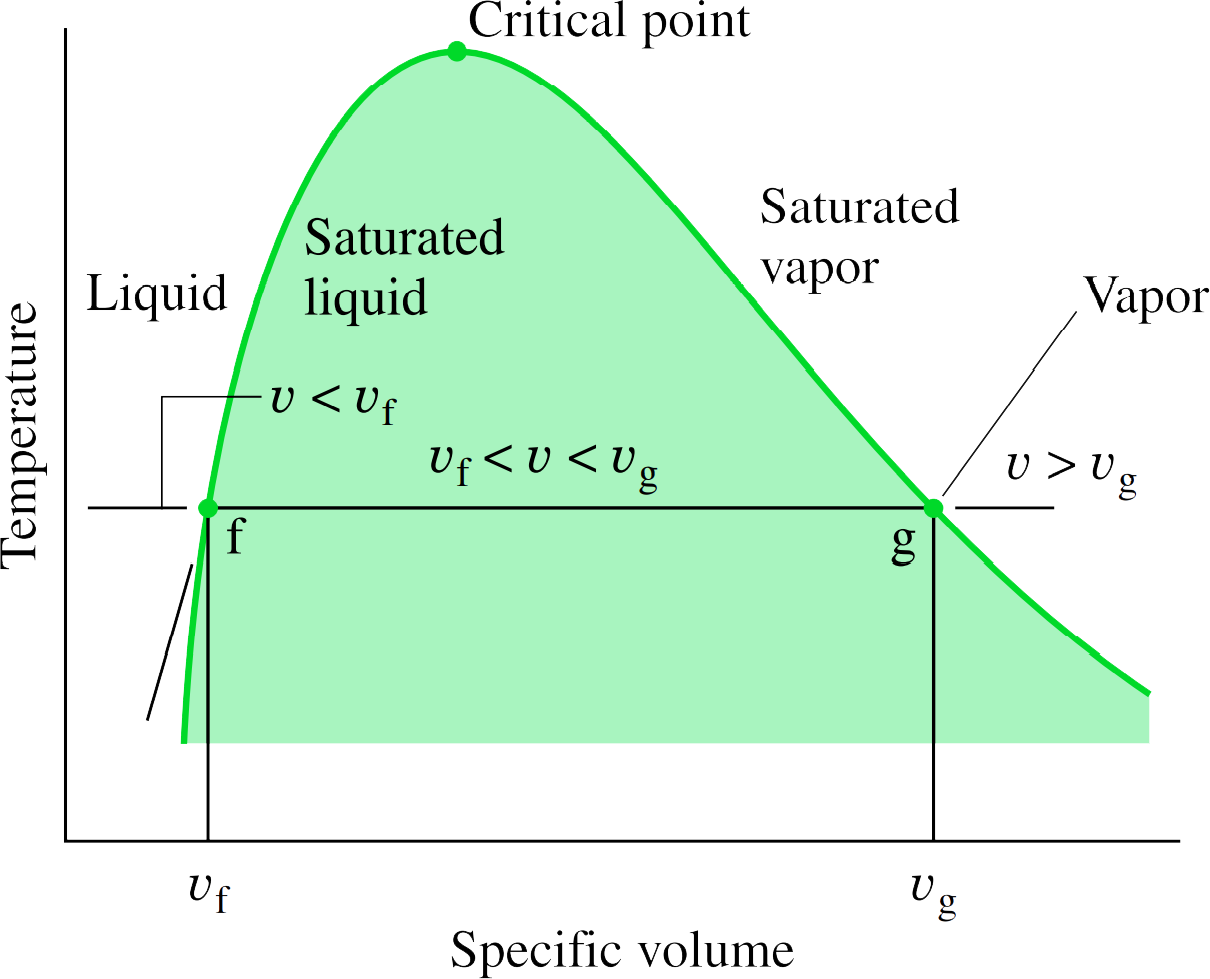
\includegraphics[height = 5cm]{D. Tv.png}
                    \caption{Diagrama Temperatura Volume}
                \end{figure}
\newpage

    \section{Modelagem de Comportamentos}
        \paragraph{Definição}Diferentes modelos matemáticos podem ser aplicados aos sistemas termodinâmicos, permitindo solucionar problemas para substâncias e valores não tabelados.

        \subsection{Substâncias Incompressíveis}
            \paragraph{Definição}Substâncias com volume específico próximo a constante e líquidos comprimidos próximos a saturação, sem mudar de fase, não alteram suas propriedades ao longo do processo. Dessa maneira pode-se utilizar as aproximações:
                \[
                    \boxed{c_{\text{v}} = \diffp{u}{T}\Big|_{\text{v}} \approx \diff{u}{T}} \hspace{5mm}
                    \boxed{c = c_{\text{v}} = c_{\text{p}}} \hspace{5mm}
                    \boxed{c_{\text{p}} = \diffp{h}{T}\Big|_{\text{p}} \approx \diff{u}{T}}
                \]
            Assim, obtém-se a equação abaixo que poderá ser aproximada caso o calor específico seja constante. Caso o atrito seja desprezível, pode-se desconsiderar qualquer aquecimento da substância.
                \[
                    \boxed{u_{2} - u_{1} \approx c (T_{2} - T_{1})} \hspace{5mm}
                    \boxed{h_{2} - h_{1} \approx c (T_{2} - T_{1}) + v(p_{2} - p_{1})}
                \]

        \subsection{Gás Ideal}
            \paragraph{Definição}Gases possuem \textbf{Fator de Compressibilidade}, determindado experimentamente, permitindo predizer seu comportamento. Formalmente definido pela seguinte relação:
                \[\boxed{Z = \frac{pv}{RT}}\]
            Todo gás se comportará como ideal a medida que a pressão ao qual está submetido se aproximar de zero. Na hipótese de gás ideal, $Z = 1$, teremos a seguinte relação para tais substâncias:
                \[
                    \boxed{pv = RT}
                \]
            Onde:
                \begin{enumerate}[noitemsep]
                    \item \textbf{Pressão}: $p$ em [Pa];
                    \item \textbf{Volume Específico}: $v$ em [m\textsuperscript{3}/kg];
                    \item \textbf{Temperatura}: $T$ em [K];
                    \item \textbf{Volume}: $V$ em [m\textsuperscript{3}];
                \end{enumerate}
            Neste caso, diferentemente da aplicação química, será necessário calcular a constante específica do gás desejado. Formalmente descrito pelas seguintes equações:
                \[
                    \boxed{R = 8,314 \hspace{2.5mm} \frac{\text{J}}{\text{mol K}}} \hspace{5mm}
                    \boxed{R_{\text{gás}} = \frac{R}{M_{\text{gás}}}} \hspace{5mm}
                    \boxed{R_{\text{ar}} = 287,053 \hspace{2.5mm} \frac{\text{J}}{\text{kg K}}}
                \]
            Onde: 
                \begin{enumerate}[noitemsep]
                    \item \textbf{Constante Universal dos Gáses}: $\overline{R}$ em [J/mol K];
                    \item \textbf{Constante do Gás}: $R$ em [J/kg K];
                    \item \textbf{Massa Molar}: $M$ em [kg/mol];
                \end{enumerate}

            \paragraph{Calor Específico}Nessa hipótese as equações relacionadas ao calor específico, a pressão e a volume constante podem ser reescritas e associadas como segue:
                \[\boxed{c_{\text{p}}(\text{T}) = c_{\text{v}}(\text{T}) + R}\]
            Aplicando a razão entre o calor específico a volume constante e a pressão constante, respectivamente, temos:
                \[
                    \boxed{c_{\text{v}}(\text{T}) = \frac{R}{k - 1}} \hspace{5mm}
                    \boxed{c_{\text{p}}(\text{T}) = \frac{kR}{k - 1}}
                \]
                \[
                    \boxed{u_{2} - u_{1} = c_{\text{v}}(T_{2} - T_{1})} \hspace{5mm}
                    \boxed{h_{2} - h_{1} = c_{\text{p}}(T_{2} - T_{1})}
                \]
\newpage

    \section{Dispositivos Termodinâmicos}
        \subsection{Válvulas}
            \paragraph{Definição}Dispositivos responsáveis por controlar o fluxo de fluido, através de válvulas manuais ou substâncias porosas, reduzindo a pressão e expandindo o volume.
                \begin{figure}[h]
                    \centering
                    \includegraphics[height = 2cm]{Válvula.png}
                    \caption{Válvulas}
                \end{figure}
                \[\boxed{h_{\text{in}} = h_{\text{out}}}\]
            Onde:
                \begin{enumerate}[noitemsep]
                    \item \textbf{Regime Permanente}: Desconsidera-se variações em sua energia;
                    \item \textbf{Adiabático}: Desconsidera-se trocas calor com o ambiente;
                    \item \textbf{Estático}: Desconsidera-se realização ou recebimento de trabalho;
                    \item \textbf{Energia}: Desconsidera-se variações pelas energias cinéticas e potenciais;
                \end{enumerate}

        \subsection{Trocadores de Calor}
            \paragraph{Definição}Dispositivos responsáveis pela transferência de calor entre dois líquidos, ou substâncias, reduzindo assim a temperatura do primeiro.
                \begin{figure}[h]
                    \centering
                    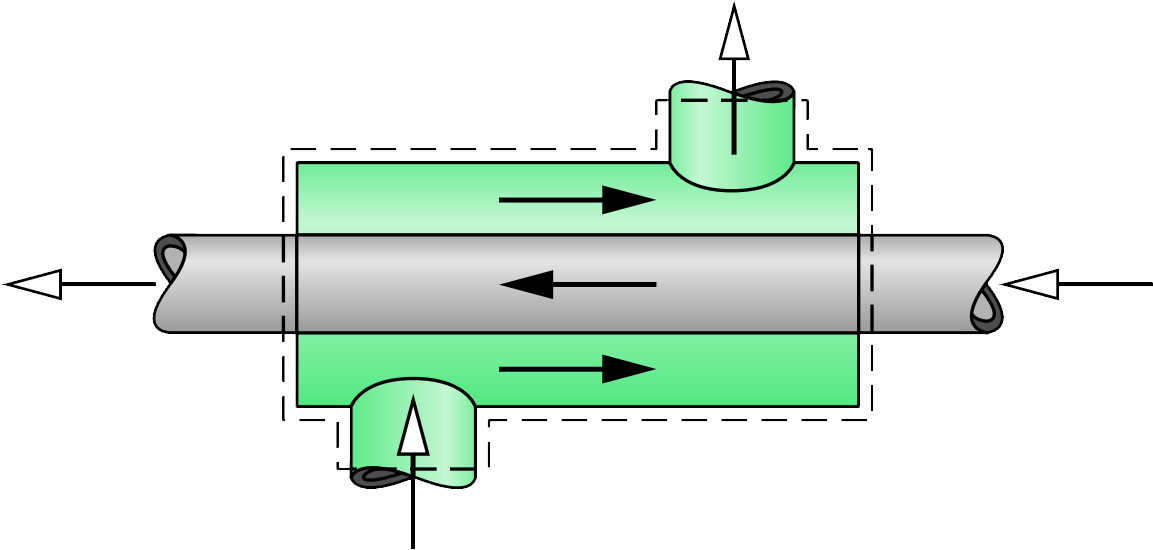
\includegraphics[height = 3cm]{Trocador de Calor a Contracorrente.png}
                    \caption{Trocadores de Calor a Contracorrente}
                \end{figure}
                \[\boxed{\sum\dot{m}_{\text{in}} h_{\text{in}} = \sum\dot{m}_{\text{out}} h_{\text{out}}}\]
            Onde:
                \begin{enumerate}[noitemsep]
                    \item \textbf{Regime Permanente}: Desconsidera-se variações em sua energia;
                    \item \textbf{Adiabático}: Desconsidera-se trocas calor com o ambiente;
                    \item \textbf{Estático}: Desconsidera-se realização ou recebimento de trabalho;
                    \item \textbf{Energia}: Desconsidera-se variações pelas energias cinéticas e potenciais;
                \end{enumerate}
\newpage

        \subsection{Redutores e Difusores}
            \paragraph{Definição}Dispositivos responsáveis, respectivamente, por incrementar a velocidade do fluido, reduzindo sua pressão ou por decrementar a velocidade do fluido, aumentando sua pressão.
                \begin{figure}[h]
                    \begin{subfigure}[t]{0.5\textwidth}
                        \centering
                        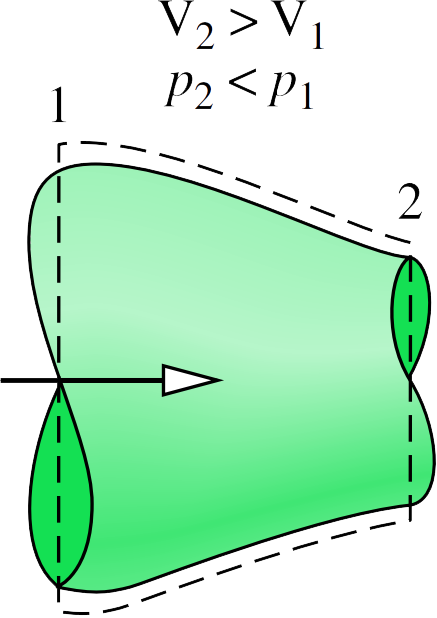
\includegraphics[height = 3cm]{Bocal Redutor.png}
                        \caption{Bocal Redutor}
                    \end{subfigure}
                    \begin{subfigure}[t]{0.5\textwidth}
                        \centering
                        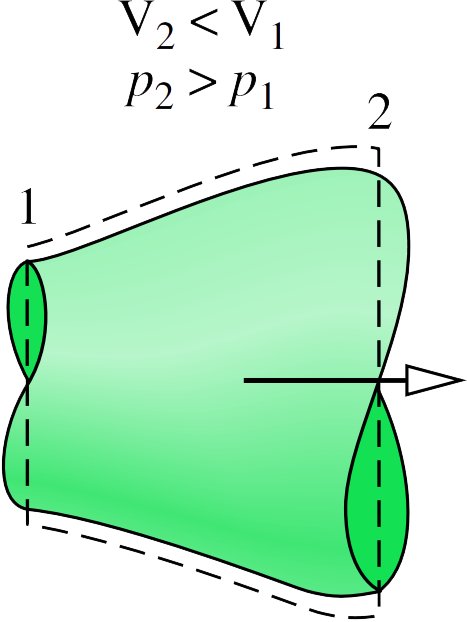
\includegraphics[height = 3cm]{Bocal Difusor.png}
                        \caption{Bocal Difusor}
                    \end{subfigure}
                    \caption{Bocais}
                \end{figure}
                \[\boxed{
                    h_{\text{in}} + \frac{V^{2}_{\text{in}}}{2} =
                    h_{\text{out}} + \frac{V^{2}_{\text{out}}}{2}}\]
            Onde:
                \begin{enumerate}[noitemsep]
                    \item \textbf{Regime Permanente}: Desconsidera-se variações em sua energia;
                    \item \textbf{Adiabático}: Desconsidera-se trocas calor com o ambiente;
                    \item \textbf{Estático}: Desconsidera-se realização ou recebimento de trabalho;
                    \item \textbf{Energia}: Desconsidera-se variações pela energia potencial;
                \end{enumerate}

        \subsection{Turbinas e Compressores}
            \paragraph{Definição}Dispositivos responsáveis, respectivamente, por gerar trabalho, reduzindo sua pressão ou por consumir trabalho, aumentando sua pressão. Geralmente operando com substâncias gasosas.
                \begin{figure}[h]
                    \begin{subfigure}[t]{0.5\textwidth}
                        \centering
                        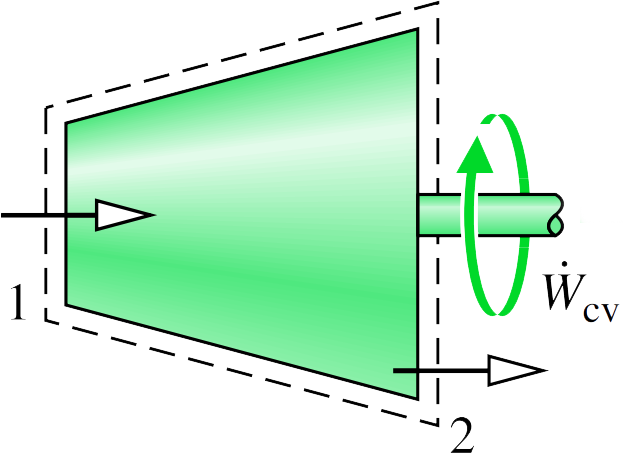
\includegraphics[height = 3cm]{Turbina.png}
                        \caption{Turbina}
                    \end{subfigure}
                    \begin{subfigure}[t]{0.5\textwidth}
                        \centering
                        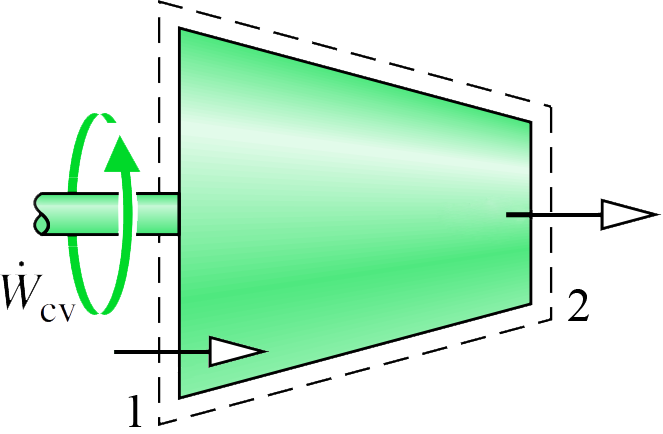
\includegraphics[height = 3cm]{Compressor de Ar.png}
                        \caption{Compressor}
                    \end{subfigure}
                    \caption{Turbinas e Compressores}
                \end{figure}
                \[\boxed{
                    \frac{\dot{W}}{\dot{m}} =
                    \frac{\dot{Q}}{\dot{m}} +
                    \left(h_{\text{in}} + \frac{V^{2}_{\text{in}}}{2}\right) -
                    \left(h_{\text{out}} + \frac{V^{2}_{\text{out}}}{2}\right)}\]
            Onde:
                \begin{enumerate}[noitemsep]
                    \item \textbf{Regime Permanente}: Desconsidera-se variações em sua energia;
                    \item \textbf{Energia}: Desconsidera-se variações pela energia potencial;
                \end{enumerate}
\newpage

        \subsection{Turbinas e Compressores Hidráulicos}
            \paragraph{Definição}Dispositivos responsáveis, respectivamente, por gerar trabalho, reduzindo sua pressão ou por consumir trabalho, aumentando sua pressão. Geralmente operando com substâncias líquidas, particularmente a água.
                \begin{figure}[h]
                    \centering
                    \includegraphics[height = 3cm]{Turbina Hidráulica.png}
                    \caption{Turbina}
                \end{figure}
                \[\boxed{
                    \frac{\dot{W}}{\dot{m}} =
                    \frac{\dot{Q}}{\dot{m}} +
                    \left(h_{\text{in}} + \frac{V^{2}_{\text{in}}}{2} + gz_{\text{in}}\right) -
                    \left(h_{\text{out}} + \frac{V^{2}_{\text{out}}}{2} + gz_{\text{out}}\right)}\]
            Onde:
                \begin{enumerate}[noitemsep]
                    \item \textbf{Regime Permanente}: Desconsidera-se variações em sua energia;
                \end{enumerate}
\newpage


    \section{1\textsuperscript{a} Lei da Termodinâmica}
        \paragraph{Definição}Qualquer alteração na energia contida no interior dum sistema ao longo do tempo virá de trocas de calor e de trabalho entre o sistema e o ambiente, respeitando a conservação energética.


        \paragraph{Convenção}Define-se que o sistema, independente de seu desempenho, deverá receber calor e realizar trabalho:
            \begin{enumerate}[noitemsep]
                \item $Q>0$: Sistema recebe calor da vizinhança;
                \item $Q<0$: Sistema fornece calor à vizinhança;
            \end{enumerate}
            \begin{enumerate}[noitemsep]
                \item $W>0$: Sistema fornece trabalho à vizinhança;
                \item $W<0$: Sistema recebe trabalho da vizinhança;
            \end{enumerate}

        \subsection{Conservação de Massa}
            \paragraph{Definição}Dentro do volume de controle a variação de massa no sistema será dada pelo balanço entre a entrada e saída do sistema. Formalmente descrita pela seguinte relação:
                \[\boxed{
                    \diff{m_{VC}}{t} = \sum_\text{in}\dot{m}_\text{in} - \sum_\text{out}\dot{m}_\text{out} 
                                       \hspace{5mm} \left[\frac{\text{kg}}{\text{s}}\right]}\]
            Onde:
                \begin{enumerate}[noitemsep]
                    \item \textbf{Vazão Mássica}: $\dot{m}$ em [kg/s];
                        \[\boxed{\dot{m} = \frac{A V}{v}}\]
                    \item \textbf{Volume Específico}: $v$ em [m\textsuperscript{3}/kg];
                    \item \textbf{Velocidade}: $V$ em [m/s];
                    \item \textbf{Área}: $A$ em [m\textsuperscript{2}];
                \end{enumerate}

        \subsection{Conservação de Energia}
            \paragraph{Definição}Dentro do volume de controle a variação de energia no sistema será dada pelo balanço entre trocas de calor, trabalho e entalpia entre o sistema e o ambiente. Formalmente descrita pela seguinte relação:
                \[\boxed{
                    \diff{E_{VC}}{t} = \dot{Q} -
                                       \dot{W} +
                                       \sum_\text{in} \dot{m}_\text{in} \left(h_\text{in}  + \frac{V^{2}_\text{in}}{2}  + gz_\text{in}\right) -
                                       \sum_\text{out}\dot{m}_\text{out}\left(h_\text{out} + \frac{V^{2}_\text{out}}{2} + gz_\text{out}\right)
                                       \hspace{5mm} \left[\text{W} = \frac{\text{kg m}^{2}}{\text{ s}^{3}}\right]}\]
            Onde:
                \begin{enumerate}[noitemsep]
                    \item \textbf{Energia}: $E$ em [J/s];
                    \item \textbf{Calor}: $\dot{Q}$ em [J/s];
                    \item \textbf{Trabalho}: $\dot{W}$ em [J/s];
                    \item \textbf{Vazão Mássica}: $\dot{m}$ em [kg/s];
                    \item \textbf{Entalpia}: $h$ em [J/kg];
                    \item \textbf{Velocidade}: $V$ em [m/s];
                    \item \textbf{Altura}: $z$ em [m];
                \end{enumerate}

        \subsection{Regime Permanente}
            \paragraph{Definição}Estado estacionário do sistema, suas propriedades permanecem constantes no tempo. Formalmente descrito pelas seguintes equações:
                \[\boxed{
                    0 = \sum_\text{in}\dot{m}_\text{in} - \sum_\text{out}\dot{m}_\text{out}}\]
                \[\boxed{
                    0 = \dot{Q} -
                        \dot{W} +
                        \sum_\text{in} \dot{m}_\text{in} \left(h_\text{in}  + \frac{V^{2}_\text{in}}{2}  + gz_\text{in}\right) -
                        \sum_\text{out}\dot{m}_\text{out}\left(h_\text{out} + \frac{V^{2}_\text{out}}{2} + gz_\text{out}\right)}\]
\newpage


    \section{2\textsuperscript{a} Lei da Termodinâmica}
        \paragraph{Definição}Qualquer processo terá sua viabilidade, ou impossibilidade, limitada pelos seguintes enunciados:
            \begin{enumerate}[noitemsep]
                \item \textbf{Clausius}: It is impossible for any system to operate in such a way that the sole result would be an energy transfer by heat from a cooler to a hotter body.
                \item \textbf{Kelvin–Planck}: It is impossible for any system to operate in a thermodynamic cycle and deliver a net amount of energy by work to its surroundings while receiving energy by heat transfer from a single thermal reservoir.
            \end{enumerate}
            \begin{figure}[h]
                \begin{subfigure}[t]{0.5\textwidth}
                    \centering
                    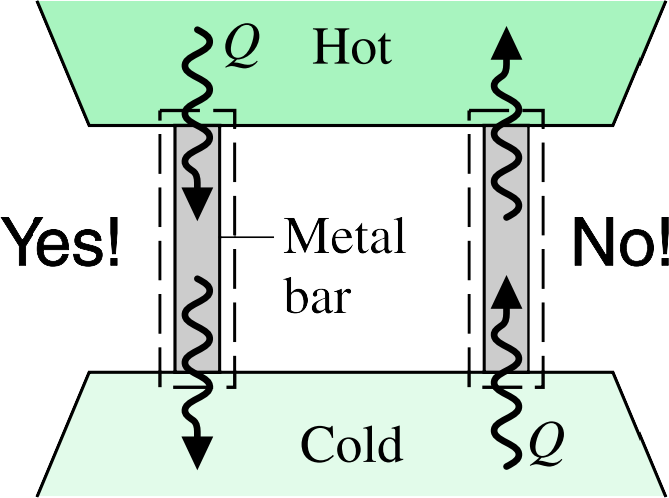
\includegraphics[height = 2cm]{Sistema de Clauss.png}
                \end{subfigure}
                \begin{subfigure}[t]{0.5\textwidth}
                    \centering
                    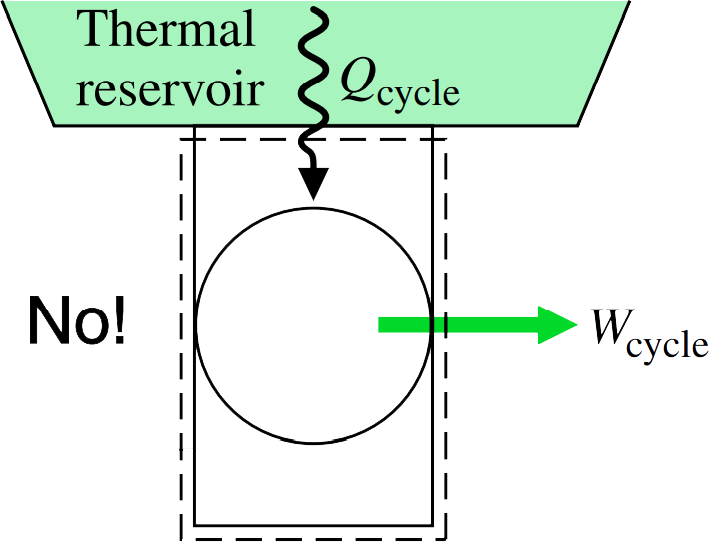
\includegraphics[height = 2cm]{Sistema Kelvin-Planck.png}
                \end{subfigure}
            \end{figure}
        Obedecendo:
            \begin{enumerate}[noitemsep]
                \item \textbf{Corolário de Carnot}: A eficiência térmica de um ciclo de potência irreversível sempre será inferior à de um ciclo de potência reversível entre os mesmos reservatórios.
                \item \textbf{Corolário de Carnot}: Todos os ciclos de potência reversíveis operando entre os mesmos reservatórios térmicos possuem a mesma eficiência térmica.
            \end{enumerate}

        \subsection{Conservação de Entropia}
            \paragraph{Definição}Dentro do volume de controle, definido para minizar as irreversibilidades internas do sistema, a variação de entropia no sistema será dada pelo balanço entre trocas de calor com a vizinhança, fluxo de entropia e as irreversibilidades do sistema. Formalmente descrita pela seguinte relação:
                \[
                    \boxed{
                        \diff{S_{VC}}{t} = \sum\limits_{i = 0}^{n} \frac{\dot{Q}_{i}}{T_{i}} +
                                           \sum\limits_\text{in} \dot{m}_\text{in}s_\text{in} -
                                           \sum\limits_\text{out} \dot{m}_\text{out}s_\text{out} +
                                           \dot{\sigma}
                    }\]
            Onde:
                \begin{enumerate}[noitemsep]
                    \item \textbf{Entropia}: $S$ em [J/K];
                    \item \textbf{Calor}: $Q$ em [J];
                    \item \textbf{Temperatura}: $T$ em [K];
                    \item \textbf{Vazão Mássica}: $\dot{m}$ em [kg/s];
                    \item \textbf{Entropia Específica}: $s$ em [J/ kg K];
                    \item \textbf{Entropia Produzida}: $\sigma$ em [J/K];
                        \begin{enumerate}[noitemsep]
                            \item $\sigma = 0$: Processo internamente reversível;
                            \item $\sigma > 0$: Processo com irreversibilidades internas;
                            \item $\sigma < 0$: Processo impossível;
                        \end{enumerate}
                \end{enumerate}

            \paragraph{Desigualdade de Clausius}Todo sistema deverá aumentar sua entropia ao final dum processo. Formalmente descrito pela seguinte relação:
                \[\boxed{\int_{\text{ciclo}} \left(\frac{\text{d}Q}{T}\right) \leq -\sigma}\]


        \subsection{Regime Permanente}
            \paragraph{Definição}Estado estacionário do sistema, suas propriedades permanecem constantes no tempo. Formalmente descrito pela seguinte equação:
            \[\boxed{
                0 = \sum\limits_{i = 0}^{n} \frac{\dot{Q}_{i}}{T_{i}} +
                    \sum\limits_\text{in} \dot{m}_\text{in}s_\text{in} -
                    \sum\limits_\text{out} \dot{m}_\text{out}s_\text{out} +
                    \dot{\sigma}}\]
\newpage

    \section{Ciclos Termodinâmicos}
        \subsection{Ciclo de Carnot}
            \paragraph{Definição}Processo cíclico ocorrendo no interior de um conjunto cílindro pistão em contanto com um reservatório térmico, percorrendo as seguintes etapas:
                \begin{figure}[h]
                    \centering
                    \includegraphics[height = 6cm]{Ciclo de Carnot Pistões.png}
                    \caption{Conjunto Ciclo de Carnot}
                \end{figure}

        \paragraph{Propriedades}Cada etapaapresentará suas particulares, descritas a seguir:
            \begin{enumerate}[noitemsep]
                \item \textbf{Compressão Adiabática}: Equilíbrio térmico do conjunto;
                \item \textbf{Expansão Isotérmica}: Recebimento de calor do reservatório;
                \item \textbf{Expansão Adiabática}: Equilíbrio térmico do conjunto;
                \item \textbf{Compressão Isotérmica}: Rejeitando calor ao reservatório;
            \end{enumerate}
            \begin{figure}[h]
                \centering
                \includegraphics[height = 6cm]{C. de Carnot Gráfico.png}
                \caption{Gráfico Ciclo de Carnot}
            \end{figure}
        Assim, considerando o gás como perfeito no interior do conjunto cílindro pitsão, pela 1\textsuperscript{a} da Termodinâmica têm-se:
            \[
                \boxed{Q = m R T \ln\frac{V_{\text{out}}}{V_{\text{in}}}} \hspace{5mm}
                \boxed{Q = m R T \ln\frac{p_{\text{in}}}{V_{\text{out}}}}\]

        \subsection{Ciclos com 1 Reservatório}
            \paragraph{Definição}Segundo \textbf{Kelvin-Planck}, será impossível, para qualquer sistema, operar em um ciclo termodinâmico capaz de entragar trabalho líquido à sua vizinhança enquanto recebe calor de um único reservatório térmico.
                \[\boxed{W_\text{ciclo} \leq 0}\]

        \subsection{Ciclos de Potência com 2 Reservatórios}
            \paragraph{Definição}Segundo \textbf{Kelvin-Planck}, um sistema em ciclo de potência com 2 reservatórios, com $Q_{C} \neq 0$, terá sua eficiência dada por:
                \begin{figure}[h]
                    \centering
                    \includegraphics[width = 8cm]{C. Aquecimento 2 Reservatórios.png}
                    \caption{Ciclo de Potência}
                \end{figure}
                \[
                    \boxed{
                        \eta =
                        \frac{|W_\text{ciclo}|}{|Q_{H}|} =
                        1 - \frac{Q_{C}}{Q_{H}}}
                    \hspace{5mm}
                    \boxed{
                        \eta_{\text{max}} =
                        1 - \frac{T_\text{{out}}}{T_\text{in}}}\]

        \subsection{Ciclos de Aquecimento e Refrigeração com 2 Reservatórios}
            \paragraph{Definição}Segundo \textbf{Clausius}, o $W_\text{ciclo} \neq 0$ pois trata-se processos não espontâneos, em que a eficiência para refrigeração e aquecimento são dadas respectivamente por:
                \begin{figure}[h]
                    \centering
                    \includegraphics[width = 8cm]{C. Resfriador 2 Reservatórios.png}
                    \caption{Ciclo de Aquecimento e Resfriamento}
                \end{figure}
                \[
                    \boxed{\beta = \frac{|Q_{C}|}{|W_\text{ciclo}|} = \frac{1}{\frac{Q_{H}}{Q_{C}} - 1}} \hspace{5mm}
                    \boxed{\gamma = \frac{|Q_{H}|}{|W_\text{ciclo}|} = \frac{1}{1 - \frac{Q_{C}}{Q_{H}}}}
                \]
                \[
                    \boxed{
                        \beta_{\text{max}} =
                        \frac{T_\text{C}}{T_\text{{H}} - T_\text{C}}}
                    \hspace{5mm}
                    \boxed{
                        \gamma_{\text{max}} =
                        \frac{T_\text{{H}}}{T_\text{{H}} - T_\text{C}}}
                \]
\newpage

    \section{Processos Isentrópicos}
        \paragraph{Definição}Aquele em que não há variação de entropia dentro do volume de controle em regime permanente. Desta maneira, sua eficiência será limitada pela geração de entropia durante o processo:
            \begin{enumerate}[noitemsep]
                \item \textbf{Compressor}: Nunca poderá consumir \textbf{Menos} potência que seu equivalente ideal;
                \item \textbf{Turbina}: Nunca poderá gerar \textbf{Mais} potência que seu equivalente ideal;
            \end{enumerate}
        Um processo será \textbf{Isentrópico} se, e somente se, este ocorrer adiabaticamente e reversivelmente.

        \subsection{Bocais}
            \paragraph{Definição}Sistemas adiabáticos que convertem pressão em energia cinética sem realização de trabalho, desconsiderando efeitos de energia potencial. Formalmente descrito pelas seguintes equações:
                \[
                    \textbf{1\textsuperscript{a} Lei: } h_{1} + \frac{V_{1}^{2}}{2} = h_{2} + \frac{V_{2}^{2}}{2} = h_{2s} + \frac{V_{2s}^{2}}{2} \hspace{10mm} 
                    \textbf{2\textsuperscript{a} Lei: } \frac{\dot{\sigma}}{\dot{m}} = s_{2} - s_{1}
                \]
            Desta maneira a eficiência será dada pela seguinte equação:
                \[\boxed{\eta = \frac{V_{2}^{2}}{V_{2s}^{2}}}\]

        \subsection{Turbinas}
            \paragraph{Definição}Sistemas adiabáticos que convertem pressão em trabalho, desconsiderando efeitos de energias cinéticas e potenciais. Formalmente descrito pelas seguintes equações: 
                \[
                    \textbf{1\textsuperscript{a} Lei: } \frac{\dot{W}}{\dot{m}} = h_{1} - h_{2} \hspace{10mm} 
                    \textbf{2\textsuperscript{a} Lei: } \frac{\dot{\sigma}}{\dot{m}} = s_{2} - s_{1}
                \]
            Desta maneira a eficiência será dada pela seguinte equação:
                \[\boxed{\eta = \frac{\dot{W}/\dot{m}}{(\dot{W}/\dot{m})_{s}} = \frac{h_{1} - h_{2}}{h_{1} - h_{2s}}}\]
                \begin{figure}[h]
                    \centering
                    \includegraphics[height = 6cm]{D. Turbina Isentrópica.png}
                    \vspace*{-4mm}
                    \caption{Diagrama $h\times s$ Turbina}
                \end{figure}

        \subsection{Compressores}
            \paragraph{Definição}Sistemas adiabáticos que convertem trabalho em pressão, desconsiderando efeitos de energias cinéticas e potenciais. Formalmente descrito pelas seguintes equações:
                \[
                    \textbf{1\textsuperscript{a} Lei: } \frac{\dot{W}}{\dot{m}} = h_{1} - h_{2} \hspace{10mm} 
                    \textbf{2\textsuperscript{a} Lei: } \frac{\dot{\sigma}}{\dot{m}} = s_{2} - s_{1}
                \]
            Desta maneira a eficiência será dada pela seguinte equação:
                \[\boxed{\eta = \frac{(\dot{W}/\dot{m})_{s}}{\dot{W}/\dot{m}} = \frac{h_{2s} - h_{1}}{h_{2} - h_{1}}}\]
                \begin{figure}[h]
                    \centering
                    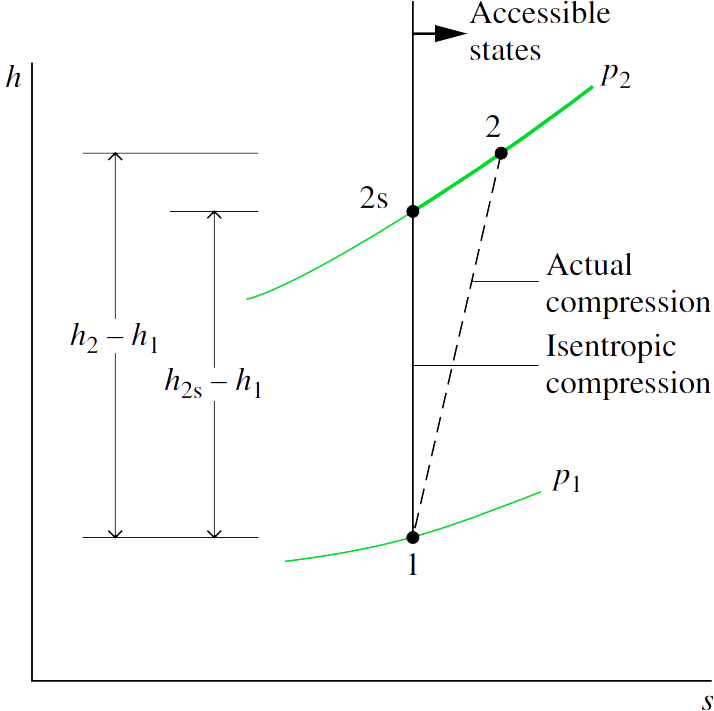
\includegraphics[height = 6cm]{D. Compressão Isentrópica.png}
                    \caption{Diagrama $h\times s$ Compressor}
                \end{figure}
\end{document}